\section{GreenOps}
\label{sec:design}

GreenOps is an online scheduler that sits above a set of cloud regions
(e.g., a multi-cluster federation) and decides, for every arriving job,
\emph{where} and \emph{when} it runs.

\paragraph{Job model.}
A job $j$ arrives at $a_j$ with runtime $d_j$, $c_j$ vCPUs, deadline $D_j$,
budget $B_j$, a set of allowed regions $A_j$ (data residency), a carbon
priority $p_j\in[0,1]$, and an input of $g_j$\,GB stored in its home
region $h_j$. Jobs belong to one of three SLA classes: \emph{strict}
(interactive, never deferred), \emph{batch}, and \emph{flexible}.

\paragraph{Cost of moving data.}
Running $j$ in $r\neq h_j$ first transfers $g_j$\,GB, taking
$\tau_{j,r}=g_j/\beta$ hours, $e_{\text{net}}\,g_j$\,kWh, and
$\pi_{\text{egress}}\,g_j$ dollars. Transfer emissions are charged at the
mean intensity of the two endpoints. Data is staged before compute
starts and occupies the network, not the target region's CPUs. Budgets
cover compute \emph{and} egress, so large inputs can make remote regions
unaffordable.

\paragraph{Candidates and hard constraints.}
At decision time $t$, GreenOps enumerates candidates $x=(r,s)$ with
$r\in A_j$, total cost $\le B_j$, start
$s\in\{t,\lceil t\rceil,\dots,\min(t{+}W,\,D_j{-}d_j{-}\tau_{j,r})\}$, and
free capacity in $r$ if $s=t$. Strict jobs only consider $s=t$.
Candidates that miss the deadline are kept only as a best-effort
fallback when no candidate can meet it.

\paragraph{Objectives.}
For each candidate GreenOps estimates three objectives:
\begin{align*}
C(x) &= \big(E_{j,r}\,\widehat{I}_r(s{+}\tau,\,s{+}\tau{+}d_j) + C^{\text{net}}_{j,r}(s)\big)\big(1+\kappa\,\sigma(s{-}t)\big)\\
K(x) &= c_j\,d_j\,\text{price}_r + \pi_{\text{egress}}\,g_j\,[r\neq h_j]\\
R(x) &= \big((s-t)/(D_j-d_j-t)\big)^{2}
\end{align*}
where $E_{j,r}$ is the job's facility energy (node power model with
PUE), $\widehat{I}_r$ is the \emph{forecast} carbon intensity averaged
over the run window, and $\sigma(h)$ is the relative forecast error at
horizon $h$. The factor $(1+\kappa\sigma)$ is a confidence gate: a
deferral must promise a saving larger than the forecast's uncertainty.
$R$ is the share of the remaining slack consumed by waiting. It is convex,
so short waits are cheap and waits close to the deadline are expensive.

\paragraph{Selection and re-planning.}
GreenOps minimises
$w_c\,p_j\,C/C_{\max} + w_k\,K/K_{\max} + w_r\,R$ over the candidates
(defaults $w=(0.6,0.2,0.2)$, $\kappa=0.5$, $W=12$\,h, selected on
held-out tuning seeds). A Pareto variant filters the non-dominated
candidates and picks a weighted Tchebycheff knee point. If the chosen start lies in the
future, the job is re-planned every hour with a fresher forecast. Jobs
that find no capacity are queued and re-considered on every resource
release. A decision evaluates at most $|R|(W{+}1)$ candidates.

\section{Methodology}
\label{sec:method}

\paragraph{Simulator.}
A discrete-event simulator built on SimPy~\cite{simpy} models regions as
pools of 16-vCPU nodes with per-node idle/peak power, PUE, price, and an
hourly carbon trace. Emissions are charged using the \emph{actual}
intensity averaged over each job's execution window, plus transfer
emissions. Late jobs are run and recorded with their tardiness, and
infeasible jobs are rejected explicitly, so no job is ever dropped silently.

\paragraph{Regions and carbon data.}
We use three regions spanning the trade-off space: India (cheap, coal-heavy),
Germany (mid-price, highly variable), and Norway (expensive,
hydro). Each has 80 nodes (1{,}280 vCPU). Hourly intensities for Germany
and Norway are derived from the 15-minute generation mix published by
Energy-Charts~\cite{energycharts} and IPCC AR5 lifecycle emission
factors~\cite{ipcc2014annex}. India has no free hourly data source, so
its trace is \emph{modelled}, calibrated to the CEA baseline
database~\cite{cea2023baseline}. We use two four-week periods, January
and July 2024 (\autoref{fig:setting}).

\begin{figure*}[t]
  \centering
  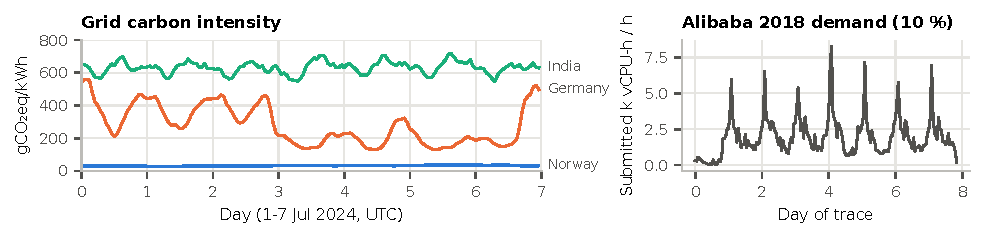
\includegraphics[width=\textwidth]{figures/fig_setting}
  \caption{Left: hourly carbon intensity of the three regions in the first
    week of July 2024 (India modelled). Right: CPU demand submitted per hour
    in the 10\,\% Alibaba sample, showing the trace's real bursts.}
  \label{fig:setting}
\end{figure*}

\paragraph{Forecasts.}
Schedulers see forecasts with error
$\widehat{I}=I\,(1+\sigma(h)\,z)$, where $\sigma(h)=\epsilon\sqrt{\min(h,24)/24}$
and $z$ is an AR(1) process ($\rho=0.7$). We set $\epsilon=0.15$ by
comparing National Grid ESO's published forecasts with actual
values for Great Britain over the same periods (relative RMSE
0.11--0.15, lag-1 autocorrelation 0.62--0.69)~\cite{ngeso}.

\paragraph{Workload.}
We replay the Alibaba cluster trace v2018~\cite{guo2019alibaba}
(4{,}000 machines, 8~days), aggregating its 14.3\,M task records into jobs.
Jobs shorter than five minutes are dropped: they are 88\,\% of jobs but
only 9\,\% of CPU-time. This leaves 450\,k jobs (median runtime 8.3\,min,
p99 1.6\,h, median 8 vCPU, capped at 64). Each seed samples 10\,\% of
these jobs ($\approx$45\,k), which gives about 50\,\% mean utilisation with
the trace's real diurnal bursts. The trace carries no SLA or data
annotations, so, as in~\cite{wiesner2021wait}, we assign them
synthetically:
\begin{itemize}
\item SLA classes and deadline slack: 30\,\% strict (0.25--1\,h),
  40\,\% batch (2--8\,h) and 30\,\% flexible (8--24\,h).
\item Home regions are uniform across regions, and 25\,\% of jobs are
  pinned to their home region.
\item Input size is $g_j = c_j d_j \cdot \gamma \cdot \text{LogNormal}(0,1)$,
  with $\gamma=1$\,GB per core-hour by default and swept in \S\ref{sec:gravity}.
\item Network energy is 0.005\,kWh/GB, extrapolated from~\cite{aslan2018network};
  egress costs \$0.02/GB and bandwidth is 1\,Gbit/s.
\end{itemize}

\paragraph{Policies.}
We compare GreenOps against eight policies:
\begin{itemize}
\item \textbf{Round Robin} and \textbf{Cost Only}: carbon-agnostic.
\item \textbf{Greenest Region}: greedy spatial shifting.
\item \textbf{Temporal Green}: carbon-greedy spatio-temporal search that
  trusts the forecast and ignores cost, transfer and SLA risk.
\item \textbf{Wait Awhile}: the non-interruptible temporal-shifting
  strategy of Wiesner et al.~\cite{wiesner2021wait}. Jobs stay in their
  home region and start in the cleanest forecast window before their
  deadline.
\item \textbf{Online Threshold}: a forecast-free reservation-price policy.
  A job runs once some eligible region's current intensity, including
  movement carbon, falls below $\sqrt{LU}$; otherwise it waits until its
  latest start. This threshold rule~\cite{elyaniv2001search} is the
  building block of the competitive spatio-temporal algorithms of
  Lechowicz et al.~\cite{lechowicz2024soad}. We implement the plain,
  non-learning-augmented variant.
\item Two GreenOps ablations: \textbf{spatial-only} ($W=0$) and
  \textbf{transfer-unaware}, which ignores data movement when deciding
  but is still charged for it.
\end{itemize}
All policies share the same capacity, budget and residency constraints.
We report means over 6 seeds $\times$ 2 seasons (12 paired runs per policy)
and test differences with a paired sign-flip permutation test.
